\part{Connect Four}

\begin{figure}
    \begin{center}
        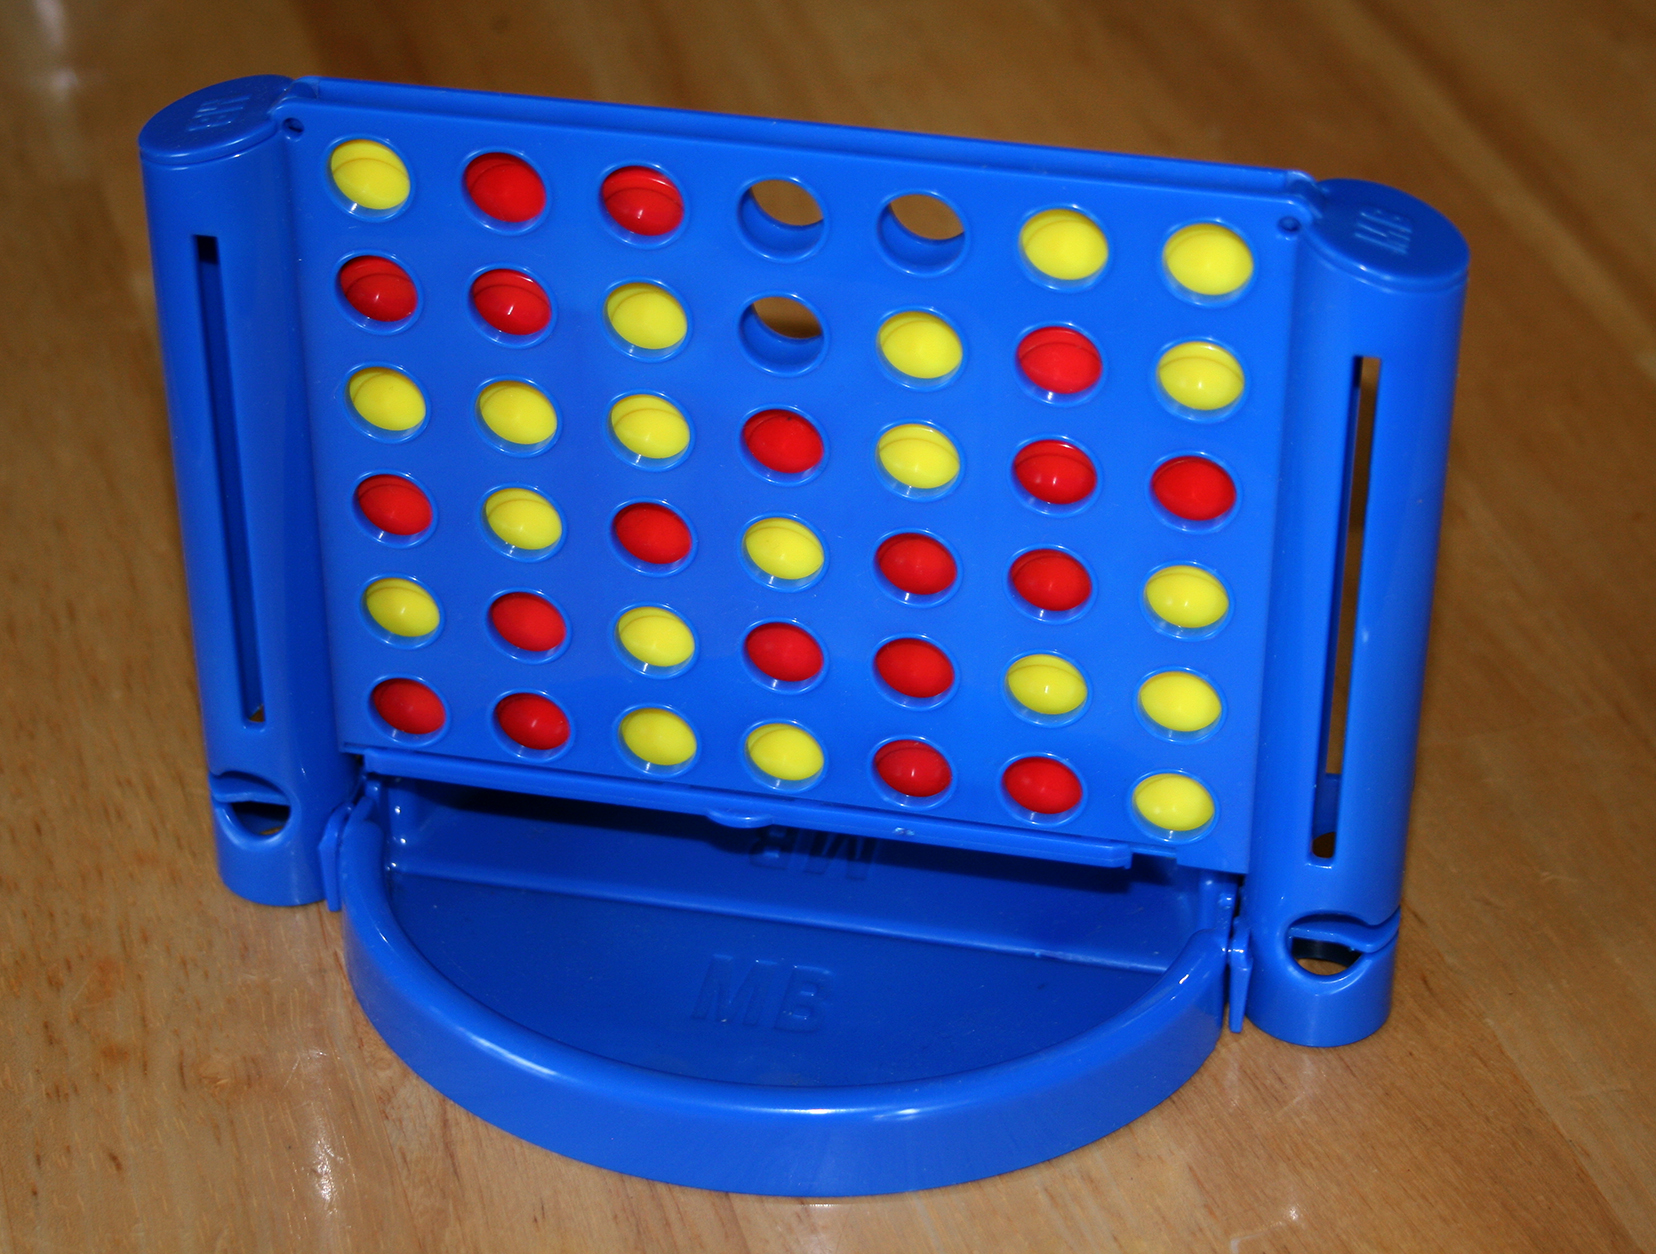
\includegraphics[width=0.6\textwidth]{connect_4.jpg}
    \end{center}
    \caption{A \emph{Connect~Four} board.
        The red player has won the game with a diagonal line starting in the lower left corner.
        Image from \protect\url{https://commons.wikimedia.org/wiki/File:Connect_Four.jpg}.}
    \label{fig:connect_4}
\end{figure}

In this part, you will implement a version of the board game \emph{Connect~Four} (Milton Bradley, 1974); see Figure~\ref{fig:connect_4}.
This is a 2-player game, in which players take turns dropping coloured counters into the top of an upright grid.
The counter falls into the lowest unoccupied space in the chosen column.
The winner is the first player to make a horizontal, vertical or diagonal line of four counters of her colour.

\section{} \label{core-b-first}

\textbf{Implement} the method \lstinline{Board::performMove}.
This method should simulate the player dropping a counter into the top of the given column \lstinline{x};
i.e.\ it should determine the lowest unoccupied square
(the largest value of \lstinline{y} such that \lstinline{getSquare(x, y) == 0})
and place the player's counter there.
It should return \lstinline{false} if the column is full, otherwise it should return \lstinline{true}.

\section{}

Algorithm~\ref{alg:b_checkline} checks for a single row of $4$ counters on the board.
The coordinates $s_x, s_y$ give the starting point of the line,
and $d_x, d_y$ (which should both be $-1$, $0$ or $+1$) give the direction.
For example $s_x=1, s_y=2, d_x=1, d_y=0$ checks the line starting at position $(1,2)$
and moving horizontally to the right.

\textbf{Implement} this algorithm as the method \lstinline{Board::checkLine} in \texttt{Board.cpp}.

\begin{algorithm}[t]
\begin{algorithmic}
    \Procedure{CheckLine}{board, $s_x$, $s_y$, $d_x$, $d_y$}
        \If{$\text{board}[s_x, s_y]$ is empty}
            \State \textbf{return} false
        \EndIf
        \For{$i = 1, 2, 3$}
            \State $t_x \gets s_x + d_x \times i$
            \State $t_y \gets s_y + d_y \times i$
            \If{$t_x, t_y$ is outside the bounds of the board}
                \State \textbf{return} 0
            \ElsIf{$\text{board}[t_x, t_y] \neq \text{board}[s_x, s_y]$}
                \State \textbf{return} 0
            \EndIf
        \EndFor
        \State \textbf{return} $\text{board}[s_x, s_y]$
    \EndProcedure
\end{algorithmic}
\caption{An algorithm for checking the presence of a single line on the Connect~Four board.}
\label{alg:b_checkline}
\end{algorithm}

\section{}

Given the above function, it is possible to check the entire board for a winning line as follows.
Loop through each square on the board.
For each square, use $\Call{CheckLine}$ to check for the following four lines:
\begin{itemize}
\item A horizontal line ($d_x=1, d_y=0$)
\item A vertical line ($d_x=1, d_y=0$)
\item A diagonal line ($d_x=1, d_y=1$)
\item A diagonal line in the other direction ($d_x=1, d_y=-1$)
\end{itemize}
If $\Call{CheckLine}$ returns true for any of these, then the winner is the player who owns the square
currently being considered.
If $\Call{CheckLine}$ never returns true for any square on the board, then there is no winner.

\textbf{Implement} this algorithm as the method \lstinline{Board::checkWin} in \texttt{Board.cpp}.

\section{} \label{core-b-last}

\textbf{Implement} the main loop of the game, structured
according to the flowchart shown in Figure~\ref{fig:flowchart_b}.

\begin{figure}
\begin{center}
\begin{tikzpicture}[node distance=1.5cm]
\node (start) [startstop] {Start};
\node (init) [process, below of=start] {Current player = 1};
\node (displayboard) [io, below of=init] {Show board};
\node (entermove) [io, below of=displayboard] {Select column};
\node (domove) [process, below of=entermove] {Perform move in selected column};
\node (iswin) [decision, below of=domove, yshift=-0.5cm] {Is there a winner?};
\node (youwin) [io, below of=iswin, yshift=-0.5cm] {Print winner};
\node (stopwin) [startstop, below of=youwin] {Stop};
\node (switchplayer) [process, right of=iswin, xshift=3cm] {Switch \mbox{current} player};
\draw [arrow] (start) -- (init);
\draw [arrow] (init) -- (displayboard);
\draw [arrow] (displayboard) -- (entermove);
\draw [arrow] (entermove) -- (domove);
\draw [arrow] (domove) -- (iswin);
\draw [arrow] (iswin) -- node[anchor=east] {yes} (youwin);
\draw [arrow] (youwin) -- (stopwin);
\draw [arrow] (iswin) -- node[anchor=south] {no} (switchplayer);
\draw [arrow] (switchplayer) |- (displayboard);
\end{tikzpicture}
\end{center}
\caption{Flowchart for the Connect 4 game.}
\label{fig:flowchart_b}
\end{figure}

\section{Stretch goal} \label{stretch-b}

The Wikipedia page for Connect~Four lists several variants of the game with modified rules (\url{https://en.wikipedia.org/wiki/Connect_Four#Rule_variations}).

\textbf{Implement} a new program, based on your Connect~Four program, implementing a rule variant of your choice.
